\begin{figure}[h]
  %\centering
  \begin{subfigure}[b]{0.4\textwidth}
    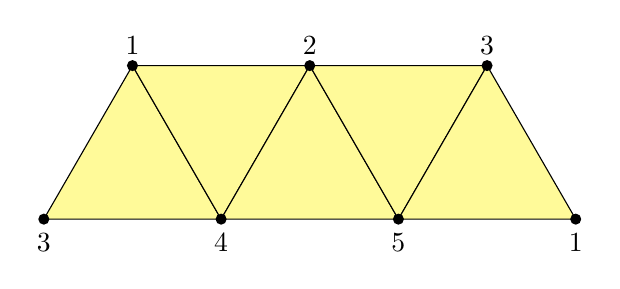
\begin{tikzpicture}
    % Define the length of the side of the triangle
    \def\side{2.251666}

    % Draw the equilateral triangle centered at (0,0)
    %\filldraw[fill=yellow!40] (90: \side) -- (210: \side) -- (330: \side) -- cycle;

    \filldraw[fill=yellow!40] (0, 0) -- (\side, 0) -- (1/2 * \side, \side * 0.8660254) -- cycle;
    \filldraw[fill=yellow!40] (\side, 0) -- (1/2 * \side, \side * 0.8660254) -- (\side * 3/2, \side * 1.732051 / 2) -- cycle;
    \filldraw[fill=yellow!40] (\side, 0) -- (2 * \side, 0) -- (\side * 3/2, \side * 1.732051 / 2) -- cycle;
    \filldraw[fill=yellow!40] (\side * 2, 0) -- (5/2 * \side, \side * 0.8660254) -- (\side * 3/2, \side * 1.732051 / 2) -- cycle;
    \filldraw[fill=yellow!40] (5/2 * \side,  \side * 0.8660254) -- (2 * \side, -0) -- (3 * \side, -0) -- cycle;
    

    % Connect the center with all three vertices
    %\draw (0,0) -- (90: \side);
    %\draw (0,0) -- (210: \side);
    %\draw (0,0) -- (330: \side);

    %\draw (0, -1/2) -- (3, 4);

    % Label the vertices and the center
    \node at (1/2 * \side,  \side * 0.8 + 0.4) {1};
    \node at (3/2 * \side,  \side * 0.8 + 0.4) {2};
    \node at (5/2 * \side,  \side * 0.8 + 0.4) {3};
    \node at (0, -0.3) {3};
    \node at (\side, -0.3) {4};
    \node at (2 * \side, -0.3) {5};
    \node at (3 * \side, -0.3) {1};
    %\node at (-0.2,0) [below right] {4}; % You can adjust the position of this label


    % Optionally, mark the center
    \fill (0, 0) circle (2pt);  % Vertex 4
    \fill (1/2 * \side, \side * 0.8660254) circle (2pt); % Vertex 1
    \fill (3/2 * \side, \side * 0.8660254) circle (2pt);
    \fill (5/2 * \side, \side * 0.8660254) circle (2pt);
    \fill (\side, 0) circle (2pt);
    \fill (2 * \side, 0) circle (2pt);
    \fill (3 * \side, -0) circle (2pt);
\end{tikzpicture}
\caption{$\LL$.}%
\end{subfigure}
\qquad\qquad
\begin{subfigure}[b]{0.4\textwidth}
    \begin{tikzpicture}
    % Define the length of the side of the triangle
    \def\side{2.251666}

    % Draw the equilateral triangle centered at (0,0)
    %\filldraw[fill=yellow!40] (90: \side) -- (210: \side) -- (330: \side) -- cycle;

    %\draw[draw=none,fill=white, fill opacity=1] (0, 0) -- (\side, 0) -- (1/2 * \side, \side * 0.8660254) -- cycle;
    
    %\draw (\side, 0) -- (1/2 * \side, \side * 0.8660254) -- (\side * 3/2, \side * 1.732051 / 2) -- cycle;
    \draw (\side, 0) -- (2 * \side, 0);
    
    \draw (0, 0) -- (\side, 0);
   % \draw[white] (\side,0) -- (1/2 * \side, \side * 0.8660254);
    \draw (1/2 * \side, \side * 0.8660254) -- (3/2 * \side, \side * 0.8660254);
    
    \draw (\side * 3/2, \side * 1.732051 / 2) -- (5/2 * \side, \side * 0.8660254);
    \draw (2 * \side, -0) -- (3 * \side, -0);

    
    % Connect the center with all three vertices
    %\draw (0,0) -- (90: \side);
    %\draw (0,0) -- (210: \side);
    %\draw (0,0) -- (330: \side);

    %\draw (0, -1/2) -- (3, 4);

    % Label the vertices and the center
    \node at (1/2 * \side,  \side * 0.8 + 0.4) {1};
    \node at (3/2 * \side,  \side * 0.8 + 0.4) {2};
    \node at (5/2 * \side,  \side * 0.8 + 0.4) {3};
    \node at (0, -0.3) {3};
    \node at (\side, -0.3) {4};
    \node at (2 * \side, -0.3) {5};
    \node at (3 * \side, -0.3) {1};
    %\node at (-0.2,0) [below right] {4}; % You can adjust the position of this label


    % Optionally, mark the center
    \fill (0, 0) circle (2pt);  % Vertex 4
    \fill (1/2 * \side, \side * 0.8660254) circle (2pt); % Vertex 1
    \fill (3/2 * \side, \side * 0.8660254) circle (2pt);
    \fill (5/2 * \side, \side * 0.8660254) circle (2pt);
    \fill (\side, 0) circle (2pt);
    \fill (2 * \side, 0) circle (2pt);
    \fill (3 * \side, -0) circle (2pt);
\end{tikzpicture}
\caption{$\KK$.}%
  \end{subfigure}
\caption{Simplicial complexes $\KK\hookrightarrow \LL$ associated with Example \ref{ex_2}.}
\label{fig_mobius}
\end{figure}